\documentclass[]{beamer}
\graphicspath{{Images/}{./}}
\usepackage{graphicx} % Required for inserting images
\usetheme{Madrid}
\usefonttheme{default}
\usepackage{palatino}
\usepackage{booktabs}
\usepackage[default]{opensans}
\usepackage{tabularx}
\usepackage{makecell}
\usepackage{amsmath}
\useinnertheme{circles}

%START PRESENTASI%
\title[Rekrutmen Asisten LPOSI ITB 2023]{Tutorial Simulation}
\subtitle{Discrete Theoretical Probability Distribution}
\author[Samuel Gibson Phang]{Samuel Gibson Phang}
\institute[14423011]{14423011 \\ \smallskip }
\date[\today]{Rekrutmen Asisten LPOSI ITB 2023\\ \today}
\date{\today}

\begin{document}

\begin{frame}
	\titlepage
\end{frame}

\begin{frame}
	\frametitle{Daftar Isi}
    \tableofcontents
\end{frame}

\section{Overview Materi}

\subsection{Uniform Distribution}

\begin{frame}{Definisi}
\frametitle{Uniform Distribution}
    Misalkan sebuah peubah acak memiliki nilai $X_1, X_2, \dots, X_k$ dengan peluang yang sama. Maka distribusi seragam diskrit didefinisikan sebagai berikut : 
    
    \bigskip
        \begin{equation*}
            f(x; k) =
            \begin{cases}
            \frac{1}{k}, & \text{untuk } x_1, x_2, \dots,x_k\\
            0, & \text{untuk lainnya}
        \end{cases}
    \end{equation*}
    \bigskip
    
    Rataan dan variansi untuk distribusi seragam diskrit adalah sebagai berikut
    
    \bigskip
        \begin{equation}
        \mu = \frac{\sum_{i=1}^{k} x_{i}}{k} \qquad \sigma^2 = \frac{\sum_{i=1}^{k} (x_{i} - \mu)^2}{k}
        \end{equation}
\end{frame}

\subsection{Binomial Distribution}

\begin{frame}{Proses Bernoulli}
    \frametitle{Binomial Distribution}
    \framesubtitle{Proses Bernoulli}
    Distribusi binomial didasarkan pada proses Bernoulli. Sifat-sifat proses Bernoulli adalah sebagai berikut :
    \bigskip
    \begin{enumerate}
        \item Eksperimen terdiri atas $n$ \textbf{percobaan yang berulang}
        \item Setiap percobaan memberikan hasil yang dapat diklasifikasikan sebagai \textbf{sukses} atau \textbf{gagal}
        \item \textbf{Peluang atas sukses} yang dinotasikan sebagai $p$ \textbf{bernilai tetap} dalam setiap percobaan
        \item Setiap percobaan bersifat \textbf{independen} (tidak bergantung pada pengujian sebelumnya)  
    \end{enumerate}
   
\end{frame}

\begin{frame}{Definisi}
    \frametitle{Binomial Distribution}
    \framesubtitle{Definisi}
    Suatu percobaan Bernoulli dapat menghasilkan sukses dengan peluang $p$ dan gagal dengan peluang $q = 1-p$. Maka distribusi peluang dari peubah acak binomial $X$, yaitu jumlah sukses dari $n$ usaha yang independen adalah :
    \bigskip
    \begin{equation*}
        P(X=x) = b(x; n, p) = \binom{n}{x} p^x q^{n-x}
    \end{equation*}
   \bigskip
   dengan 
   \bigskip
   \begin{equation*}
       \binom{n}{x} = \frac{n!}{x!(n-x)!}
   \end{equation*}
   \bigskip
   
   Rataan dan variansi untuk distribusi binomial adalah sebagai berikut
    \begin{equation*}
        \mu = np \qquad \sigma^2 = npq
    \end{equation*}
\end{frame}

\begin{frame}{Distribusi Kumulatif}
    \frametitle{Binomial Distribution}
    \framesubtitle{Distribusi Kumulatif}
    Seringkali dalam soal biasanya kita diminta untuk menghitung distribusi kumulatif $P(x\le a) $ atau $P(a\le x\le b) $
    \bigskip
    \begin{equation*}
        P(x \le a) = \sum_{x=0}^a \binom{n}{x} p^x q^{n-x}
    \end{equation*}
    \begin{equation*}
        P(a \le x \le b) = \sum_{x=a}^b \binom{n}{x} p^x q^{n-x}
    \end{equation*}
    \bigskip
    
    Untuk itu, telah disiapkan Tabel Distribusi Kumulatif Binomial pada Tabel A.1 Appendix Buku Walpole
\end{frame}

\begin{frame}{Tabel Distribusi}
	\frametitle{Binomial Distribution}
	\framesubtitle{Tabel Distribusi}
	\begin{figure}
		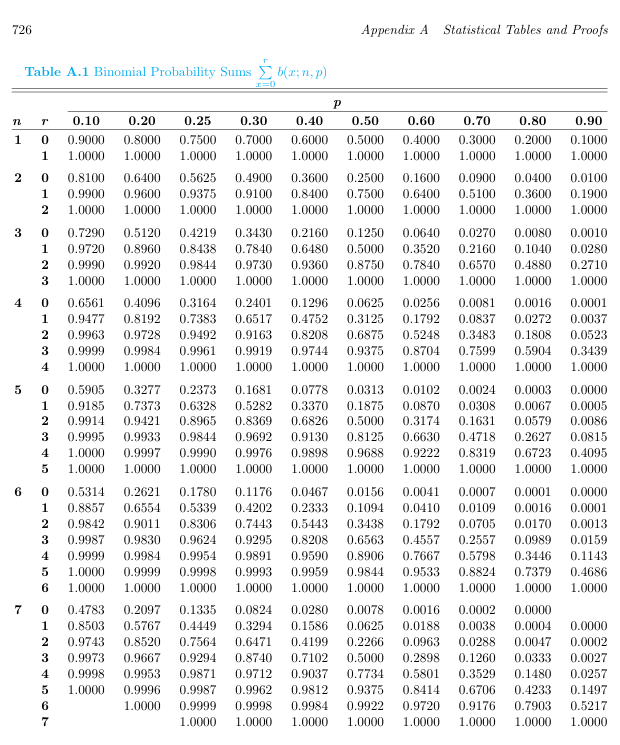
\includegraphics[width=0.4\linewidth]{Isian grafik/Tabel Binomial.png}
		\caption{Tabel Distribusi Binomial}
	\end{figure}
\end{frame}

\subsection{Negative Binomial Distribution}


\begin{frame}{Definisi}
    \frametitle{Negative Binomial Distribution}
    \framesubtitle{Definisi}
    Pada distribusi binomial negatif, alih-alih kita ingin mencari probabilitas munculnya $x$ sukses dalam $n$ percobaan, dimana $n$ bernilai tetap, kita sekarang ingin mencari probabilitas munculnya sukses ke-$k$ pada percobaan ke-$n$ 
    
    \bigskip
    
    Jika percobaan yang saling bebas dilakukan berulang kali menghasilkan sukses dengan peluang $p$ dan gagal dengan peluang $q=1-p$, maka distribusi peluang acak $X$, yaitu banyaknya percobaan yang berakhir tepat pada sukses ke-$k$ adalah
    \bigskip
    \begin{equation*}
        b^*(x;k,p)=\binom{x-1}{k-1}p^kq^{x-k} \qquad x=k,k+1,k+2,\dots
    \end{equation*}
\end{frame}

\subsection{Geometric Distribution}

\begin{frame}{Definisi}
\frametitle{Geometric Distribution}
    \begin{itemize}
        \item Misalkan kita mempertimbangkan kasus khusus distribusi binomial negatif dimana $k=1$. Dari sini didapatkan distribusi probabilitas untuk jumlah percobaan yang diperlukan untuk satu keberhasilan
        \item \textbf{Definisi : }Jika percobaan yang saling bebas yang dilakukan berulang kali menghasilkan peluang sukses sebesar $p$ dan peluang gagal sebesar $q=1-p$, maka distribusi peluang acak $X$, yaitu banyaknya usaha sampai terjadinya sukses yang pertama adalah
        \begin{equation*}
            g(x;p)=pq^{x-1} \qquad x=1,2,\dots
        \end{equation*}
        \item Rataan dan variansi untuk distribusi geometrik adalah
        \begin{equation*}
            \mu=\frac{1}{p} \qquad \sigma^2 = \frac{1-p}{p^2}
        \end{equation*}
    \end{itemize}
\end{frame}

\subsection{Multinomial Distribution}    

\begin{frame}{Definisi}
    \frametitle{Multinomial Distribution}
    \framesubtitle{Definisi}
    Misalkan suatu percobaan dapat menghasilkan k macam hasil $E_1, E_2,\dots,E_k$ dengan probabilitas $p_1, p_2, \dots, p_k$, maka distribusi peluang dari peubah acak $X_1, X_2,\dots,X_k$ yang menyatakan banyak terjadinya $E_1, E_2,\dots,E_k$ dalam n usaha yang independen adalah
    \bigskip
    \begin{equation*}
    f(x_1,x_2,\dots,x_k;p_1,p_2,\dots,p_k,n) = \binom{n}{x_1,x_2,\dots,x_k}p_1^{x_1}p_2^{x_2}\dots p_k^{x_k}
    \end{equation*}
    \bigskip
    dengan
    \bigskip
    \begin{equation*}
        \sum_{i=1}^kx_i = n, \qquad \sum_{i=1}^kp_i = 1 \qquad \binom{n}{x_1,x_2, \dots, x_k}=\frac{n!}{x_1!x_2!\dots x_k!}
    \end{equation*}
\end{frame}

\subsection{Hypergeometric Distribution}

\begin{frame}{Percobaan Hipergeometrik}
    \frametitle{Hypergeometric Distribution}
    \framesubtitle{Percobaan Hipergeometrik}
    Distribusi hipergeometrik didasarkan pada \textbf{percobaan hipergeometrik} yang memiliki sifat-sifat sebagai berikut 
    \begin{enumerate}
        \item Secara acak diambil sampel sebanyak $n$ tanpa dikembalikan dari $N$ benda
        \item $k$ dari $N$ benda diklasifikasikan sebagai sukses, dan $N-k$ diklasifikasikan sebagai gagal
    \end{enumerate}
    Jumlah sukses $X$ dari percobaan hipergeometrik disebut \textbf{peubah acak hipergeometrik}
    
    \bigskip
    
    Distribusi peluang dari peubah acak hipergeometrik disebut dengan \textbf{distribusi hipergeometrik} dan dinotasikan sebagai $h(x;n,N,k)$
\end{frame}

\begin{frame}{Definisi}
    \frametitle{Hypergeometric Distribution}
    \framesubtitle{Definisi}
    Distribusi peluang dari peubah acak hipergeometrik $X$, yaitu jumlah sukses dari sampel acak berukuran $n$ yang diambil dari $N$ benda, dimana terdapat sejumlah $k$ sukses dan $N-k$ jumlah gagal adalah
    \begin{equation*}
        h(x;N,n,k) = \frac{\binom{k}{x}\binom{N-k}{n-x}}{\binom{N}{n}}, \qquad \max\{0, n - (N - k)\} \le x \le \min\{n, k\}
    \end{equation*}
    dimana $x=1,2,...,n$
    
    \bigskip
    
    Rataan dan variansi untuk distribusi hipergeometrik adalah
    \begin{equation*}
        \mu = \frac{Nk}{n} \qquad \sigma^2 = \frac{N-n}{N-1}\cdot n\cdot \frac{k}{N}(1-\frac{k}{N})
    \end{equation*}
\end{frame}

\begin{frame}{Aproksimasi Distribusi Hipergeometrik dengan Distribusi Binomial}
    \frametitle{Hypergeometric Distribution}
    \framesubtitle{Aproksimasi Distribusi Hipergeometrik dengan Distribusi Binomial}
    \begin{itemize}
        \item Jika nilai $n$ terlampau kecil dibandingkan $N$, dimana $\frac{n}{N}\le0.05$, distribusi hipergeometrik dapat diaproksimasi dengan distribusi binomial.
        \item Nilai $p$ pada distribusi binomial didekati dengan $\frac{k}{N}$ pada distribusi binomial
        \item Aproksimasi nilai $h(x;N,n,k)$ dapat dinyatakan sebagai berikut
            \begin{equation*}
            h(x;N,n,k) \approx b(x;n,\frac{k}{N})
            \end{equation*}
        \item Aproksimasi rataan dan variansi untuk distribusi hipergeometrik dengan distribusi binomial adalah 
            \begin{equation*}
                \mu = np = \frac{nk}{N} \qquad \sigma^2 = npq = n \cdot \frac{k}{N} \cdot(1-\frac{k}{N})
            \end{equation*}
    \end{itemize}
\end{frame}

\begin{frame}{Multivariate Hypergeometric Distribution}
    \frametitle{Hypergeometric Distribution}
    \framesubtitle{Multivariate Hypergeometric Distribution}
    Jika N benda dapat dipartisi menjadi $k$-sel $A_1, A_2,\dots,A_k$ yang masing-masing berisi $a_1, a_2, \dots, a_k$ benda, maka distribusi peluang acak $X_1, X_2,\dots,X_k$ yang menyatakan banyaknya benda yang terambil dari $A_1, A_2,\dots,A_k$ dalam suatu sampel acak berukuran $n$ adalah
    \begin{equation*}
        f(x_1,x_2,\dots,x_k;a_1,a_2,\dots,a_k,N,n) = \frac{\binom{a_1}{x_1}\binom{a_2}{x_2}\dots \binom{a_k}{x_k}}{\binom{N}{n}}
    \end{equation*}
    dimana
    \begin{equation*}
        \sum_{i=1}^kx_i = n, \qquad \sum_{i=1}^ka_i = N
    \end{equation*}
\end{frame}

\begin{frame}{Contoh Soal}
\frametitle{Hypergeometric Distribution}
\framesubtitle{Contoh Soal}
    \begin{block}{Soal}
    \scriptsize
        Saat MTI akan memilih ketua himpunan yang terdiri atas calon tunggal,  ditemukan bahwa 80 dari 400 daftar pemilih tetap memilih kotak kosong. Jika 5 daftar pemilih tetap dipilih secara acak dan ditanya mengenai pilihan ketua himpunan, berapa probabilitas dimana 3 diantaranya memilih kotak kosong?
    \end{block}
    \begin{exampleblock}{Pembahasan}
        Misalkan "sukses" diidentifikasikan sebagai pemilih kotak kosong. didapatkan. Asumsikan hanya terdapat 2 pilihan, yaitu memilih ketua himpunan atau kotak kosong. Berdasarkan soal, didapatkan $N=400, n=5, k=80, x=3$. Maka
        \begin{equation*}
            h(3;400.5,80) =\frac{\binom{80}{3}\binom{320}{2}}{\binom{400}{5}}=\textbf{0.0504}
        \end{equation*}
    \end{exampleblock}
\end{frame}
\subsection{Poisson Distribution}

\begin{frame}{Proses Poisson}
    \frametitle{Poisson Distribution}
    \framesubtitle{Proses Poisson}
     Distribusi Poisson merupakan distribusi yang didasarkan pada proses Poisson. Sifat-sifat proses Poisson adalah sebagai berikut
        \begin{enumerate}
            \item Jumlah hasil yang terjadi dalam satu selang waktu atau daerah tertentu bersifat independen terhadap hasil yang terjadi pada selang atau daerah lain. Dalam hal ini, proses Poisson dikatakan tidak memiliki ingatan (\textit{memoryless})
            \item Probabilitas terjadinya suatu hasil (tunggal) dalam selang waktu yang sangat pendek daerah yang sangat kecil sebanding dengan panjang selang waktu atau besarnya daerah dan tidak bergantung pada banyaknya hasil yang terjadi di luar selang atau daerah tersebut
            \item  Peluang terjadinya lebih dari satu hasil yang terjadi dalam selang waktu yang pendek dapat diabaikan (biasanya dianggap 0)
        \end{enumerate}
\end{frame}

\begin{frame}{Definisi}
    \frametitle{Poisson Distribusi}
    \framesubtitle{Definisi}
    Distribusi probabilitas peubah acak Poisson $X$, yang menyatakan banyaknya sukses yang terjadi dalam selang waktu atau daerah tertentu, dinotasikan dengan $\mu$ adalah
    \begin{equation*}
        P(x;\mu)=\frac{e^{-\mu}\mu^x}{x!} \qquad x=0,1,2,\dots
    \end{equation*}
    dimana $\mu=\lambda t$ adalah rata-rata banyaknya sukses yang terjadi per satuan waktu atau daerah tertentu, $\lambda$ adalah jumlah kejadian per satuan waktu, jarak, luas, atau volume, dan $e=2.71828$ 

    \bigskip

    Rataan dan variansi untuk distribusi Poissson adalah sama, yaitu
    \begin{equation*}
        \mu=\sigma^2=\lambda t
    \end{equation*}
\end{frame}

\begin{frame}{Distribusi Kumulatif}
    \frametitle{Poisson Distribution}
    \framesubtitle{Distribusi Kumulatif}
    Sama halnya dengan distribusi binomial, ada kalanya dalam soal biasanya kita diminta untuk menghitung distribusi kumulatif $P(x\le a) $ atau $P(a\le x\le b) $
    \begin{equation*}
        P(x\le a) = \sum_{x=0}^a \frac{e^{-\mu}\mu^x}{x!}
    \end{equation*}
    \begin{equation*}
        P(a\le x\le b) = \sum_{x=a}^b \frac{e^{-\mu}\mu^x}{x!}
    \end{equation*}
    
    \bigskip

    Untuk itu, telah disiapkan tabel distribusi kumulatif Poisson pada Appendix Tabel A.2 buku Walpole
\end{frame}

\begin{frame}{Tabel Distribusi}
	\frametitle{Poisson Distribution}
	\framesubtitle{Tabel Distribusi}
	\begin{figure}
		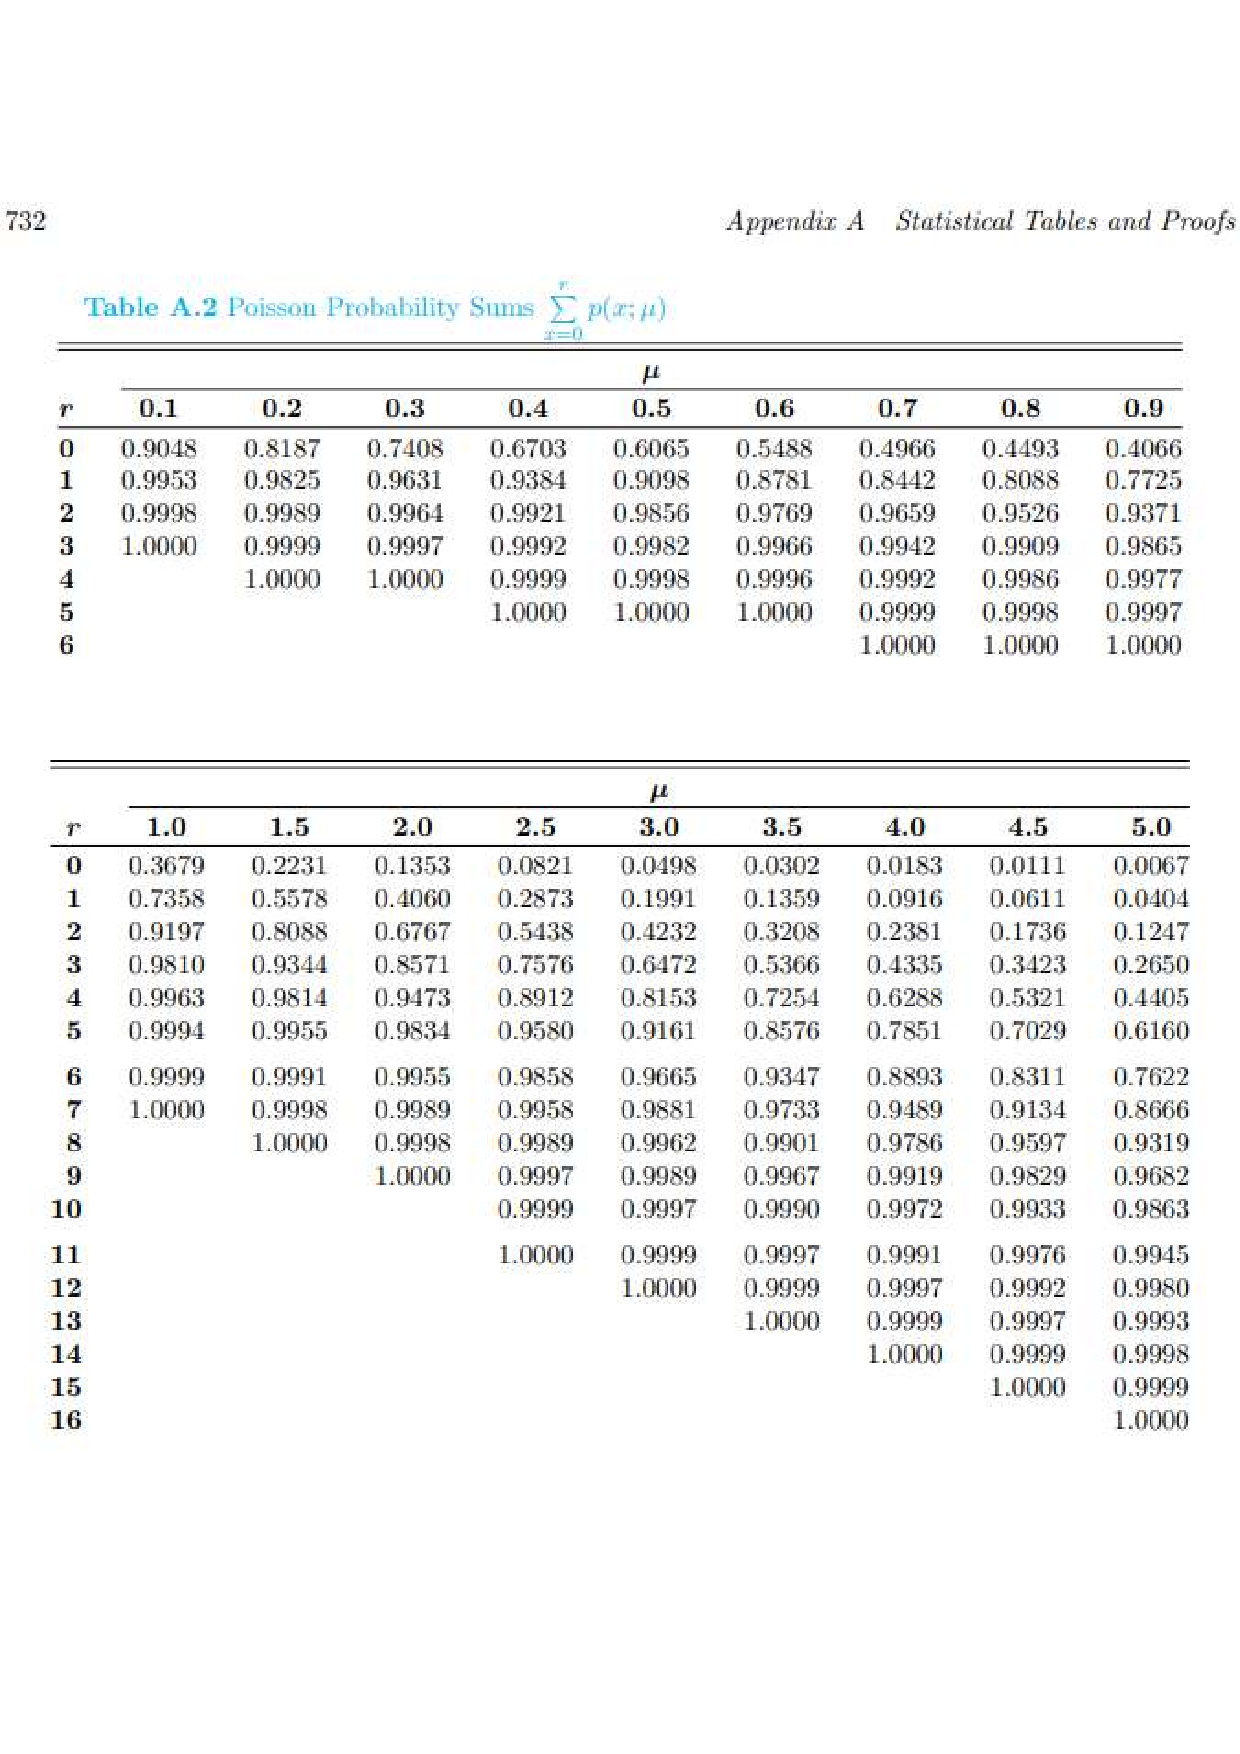
\includegraphics[width=0.4\linewidth]{Isian grafik/Screenshot 2025-11-10 221128.pdf}
		\caption{Tabel Distribusi Probablilitas Poisson}
	\end{figure}
\end{frame}

\begin{frame}{Aproksimasi Distribusi Binomial dengan Distribusi Poisson}
\frametitle{Distribusi Poisson}
\framesubtitle{Aproksimasi Distribusi Binomial dengan Distribusi Poisson}
    \begin{itemize}
        \item Pada distribusi binomial, jika nilai $n$ terlampau besar ($n\longrightarrow \infty$) dan nilai $p$ terlampau kecil ($p\longrightarrow 0$), distribusi Binomial dapat diaproksimasi dengan distribusi Poisson.
        \item Nilai $\mu$ pada distribusi Poisson didekati dengan $np$ pada distribusi Binomial
        \item Aproksimasi nilai $b(x;n,p)$ dapat dinyatakan sebagai berikut
            \begin{equation*}
            b(x;n,p) \approx p(x;np)
            \end{equation*}
    \end{itemize}
    \textbf{Catatan : } Nilai aproksimasi \alert{bukan merupakan nilai sebenarnya}, namun hanya bersifat pendekatan dan memiliki nilai \textit{error} (selisih) jika dibandingkan perhitungan dengan distribusi sebenarnya
\end{frame}

\begin{frame}{Contoh Soal}
\frametitle{Poisson Distribution}
\framesubtitle{Contoh Soal}
    \begin{block}{Soal}
		Dari sebuah data yang didapatkan melalui pengamatan persimpangan jalan, terdapat 3 kecelakaan per bulan terjadi di persimpangan tersebut. Tentukan probabilitas dimana:
        \begin{enumerate}
            \item Tepat 5 kecelakaan terjadi dalam 1 bulan.
            \item Kurang dari 3 kecelakaan terjadi dalam 1 bulan.
            \item Lebih dari 3 kecelakaan terjadi dalam 2 bulan.
        \end{enumerate}
	\end{block}
    \begin{exampleblock}{Pembahasan}
		Misalkan $t$ merupakan waktu pengamatan dalam bulan dan $\lambda=3$. Maka
        \begin{equation*}
            \mu=\lambda t = 3t
        \end{equation*}
        
	\end{exampleblock}
\end{frame}

\begin{frame}
    \begin{exampleblock}{Pembahasan}
        \begin{enumerate}
            \item Untuk $P(X=3)$ dalam 1 bulan, $\mu = (3)(1) = 3$. Maka :
            \begin{equation*}
                P(X=3)= P(3;3)=\frac{e^{-3}3^3}{3!} = 0.224
            \end{equation*}
            \item Untuk $P(X<3)$ dalam 1 bulan, $\mu = (3)(1) = 3$. Maka :
            \begin{equation*}
                P(X<3)= P(X\le 2) = \sum_{i=0}^2 P(x;3)=\frac{e^{-3}3^x}{x!} = 0.4232
            \end{equation*}
            \item Untuk $P(X>3)$ dalam 2 bulan, $\mu = (3)(2) = 6$. Maka
            \begin{equation*}
                P(X>3)= 1-P(X\le 3) = 1-\sum_{i=0}^3 P(x;6)=\frac{e^{-6}6^x}{x!} = 0.8488
            \end{equation*}
        \end{enumerate}
    \end{exampleblock}
\end{frame}
\section{Ringkasan}

\begin{frame}
	\frametitle{Review}
	\begin{table}
    \tiny
		\begin{tabular}{l | l | l | l | l}
			\toprule
			\textbf{Distribusi} & \textbf{Parameter} & \textbf{Persamaan} & \textbf{Rataan ($\mu$)} & \textbf{Variansi ($\sigma^2$)} \\
			\midrule
			Uniform & $k$ & $\frac{1}{k}$ & $ \frac{\sum_{i=1}^{k} x_{i}}{k}$ & $\frac{\sum_{i=1}^{k} (x_{i} - \mu)^2}{k}$ \\
            \hline
			Binomial & $x, n, p$ & $\binom{n}{x} p^x(1-p)^{1-x}$ & $np$ & $np(1-p)$\\
            \hline
			Negaitve Binomial & $x, n, p$ & $\binom{x-1}{k-1}p^k(1-p)^{x-k}$ \\
            \hline
            Geometric & $x, p$ & $p(1-p)^{x-1}$ & $\frac{1}{p}$ & $\frac{1-p}{p^2}$\\
            \hline
            Multinomial & $x,n,p_i$ & $\binom{n}{x_1,x_2,\dots,x_k}p_1^{x_1}p_2^{x_2}\dots p_k^{x_k}$\\
            \hline
            Hypergeometric & $x, N, n, k$ & $\frac{\binom{k}{x}\binom{N-k}{n-x}}{\binom{N}{n}}$ & $\frac{Nk}{n}$ &$ \frac{N-n}{N-1}\cdot n\cdot \frac{k}{N}(1-\frac{k}{N})$\\
            \hline
            \makecell[l]{Multivariate \\ Hypergeometric} \ & $x_i, a_i, N, n$ & $\frac{\binom{a_1}{x_1}\binom{a_2}{x_2}\dots \binom{a_k}{x_k}}{\binom{N}{n}}$ \\
            \hline
            Poisson & $x,\lambda,t$ & $\frac{e^{\lambda t}{\lambda t}^x}{x!}$ & $\lambda t$ & $\lambda t$\\
			\bottomrule
		\end{tabular}
		\caption{Ringkasan Distribusi Teoretis Diskrit}
	\end{table}
\end{frame}

\section{Soal}

\begin{frame}
\frametitle{Contoh Soal}
\tiny
    \begin{block}{Soal Bagian A}
        Tim pelatih sepakbola MTI FC. sedang mengevaluasi berbagai metrik kinerja yang berbeda. Data awal yang didapatkan adalah sebagai berikut
        \begin{itemize}
            \item Tingkat keberhasilan penalti MTI FC adalah $0.8$ per tendangan
            \item MTI FC menerima kartu kuning rata-rata sebesar $1.2$ kartu kuning per pertandingan
            \item MTI FC memiliki total 30 pemain, di mana 8 pemain di antaranya memiliki rating fisik di atas 90 (dianggap elit).
        \end{itemize}
        Pertanyaan :
        \begin{enumerate}
            \item Dalam sebuah turnamen, MTI FC bermain 5 pertandingan. Jika diasumsikan jumlah kartu kuning dan hasil penalti bersifat independen, berapakah peluang Tim MTI FC mendapatkan total tepat 3 kartu kuning selama 5 pertandingan tersebut, dengan syarat bahwa mereka juga berhasil mencetak tepat 4 gol dari 5 peluang penalti yang mereka dapatkan sepanjang turnamen?
            \item Manajemen tim memutuskan bahwa analisis kartu kuning harus diukur per paruh waktu (yaitu, per 45 menit), bukan per pertandingan (90 menit).Berapakah Variansi ($\sigma^2$) dari jumlah kartu kuning yang diterima MTI FC dalam 10 paruh waktu berturut-turut, jika diketahui bahwa tingkat kejadian kartu kuning adalah konstan?
            \item MTI FC memutuskan untuk melatih penalti baru. Mereka ingin tahu berapa jumlah minimum tendangan penalti berikutnya yang harus mereka ambil agar probabilitas keberhasilan mereka mencapai minimal 90 persen, (yaitu, $P(X \ge 1) \ge 0.90$) untuk mendapatkan setidaknya satu gol dari tendangan penalti tersebut?
            \item Manajer tim mengambil sampel 6 pemain untuk wawancara dari total 30 pemain. Pengambilan dilakukan tanpa pengembalian. Berapakah peluang bahwa manajer memilih tepat 2 pemain yang memiliki rating fisik di atas 90?
            \item Dalam suatu babak playoff, MTI FC harus memenangkan total 3 pertandingan untuk lolos ke babak berikutnya. Diketahui probabilitas MTI FC memenangkan setiap pertandingan adalah 0.6. Berapakah peluang bahwa MTI FC harus memainkan total 5 pertandingan (termasuk 3 kemenangan) untuk mencapai target tersebut?
        \end{enumerate}
    \end{block}
\end{frame}

\begin{frame}
\frametitle{Contoh Soal}
\scriptsize
    \begin{exampleblock}{Pembahasan Soal Nomor 1}
        Karena diasumsikan kedua kejadian independen, maka berlaku
        \begin{equation*}
            P(A\cap B) = P(A) \times P(B)
        \end{equation*}
        \textbf{1. Hitung probabilitas kartu kuning ($P(A)$)}
        
        \bigskip
        
        Kartu kuning mengikuti distribusi Poisson. Untuk 5 pertandingan, perlu dicari rata-rata kartu kuning untuk 5 pertandingan
        \begin{itemize}
            \item Rata-rata per pertandingan : $\mu_{pertandingan}=\lambda_{pertandingan} \times t =1.2$
            \item Rata-rata untuk 5 pertandingan : $\mu_{total}=\lambda_{pertandingan} \times t = 1.2\times 5 = 6$
        \end{itemize}
        Menggunakan distribusi Poisson($P(X=x) = \frac{e^{-\mu} \mu^x}{x!}$), didapatkan
        \begin{equation*}
            P(X=3 \text{ kartu}) = \frac{e^{-6} 6^3}{3!} = \frac{0.002479 \times 216}{6} \approx 0.0892
        \end{equation*}
    \end{exampleblock}
\end{frame}

\begin{frame}
    \scriptsize
    \frametitle{Contoh Soal}
    \begin{exampleblock}{Pembahasan Soal Nomor 1}
        \textbf{2. Hitung probabilitas penalti ($P(B)$)}

        \bigskip
        
        Penalti mengikuti Distribusi Binomial ($n=5, p=0.80$). Kita mencari $x=4$ gol. Menggunakan Rumus Binomial ($P(X=x) = \binom{n}{x} p^x (1-p)^{n-x}$), didapatkan
        \begin{equation*}
            P(Y=4 \text{ gol}) = \binom{5}{4} (0.80)^4 (1-0.80)^{5-4} \approx 0.4096
        \end{equation*}

        \textbf{3. Hitung Probabilitas Gabungan}

        \bigskip
        
        Karena kedua kejadian independen, maka
        \begin{equation*}
            P(A \cap B) = P(A) \times P(B) \approx 0.0892 \times 0.4096 \approx \mathbf{0.0365}
        \end{equation*}
        
        \bigskip
        
        Maka, peluang MTI FC mendapatkan tepat 3 kartu kuning dan mencetak 4 gol dari 5 penalti adalah sekitar 0.0365
    \end{exampleblock}
\end{frame}

\begin{frame}
    \frametitle{Contoh Soal}
    \scriptsize
    \begin{exampleblock}{Pembahasan Soal Nomor 2}
        Peluang mendapatkan Kartu Kuning berdistribusi Poisson, di mana $\mu = Var[X] = \lambda_{pertandingan} \times t$. 
        \begin{itemize}
            \item Laju kartu kuning per pertandingan (90 menit) : $\lambda_{pertandingan}$
            \item Laju kartu kuning per paruh waktu (45 menit) : $\lambda_{paruh waktu}=\frac{\lambda_{pertandingan}}{2} = \frac{1.2}{2} = 0,6$
            \item Total interval baru $(n)$ = 10 paruh waktu
            \item Rata-rata kartu kuning dalam 10 paruh waktu : $\mu_{total}=\lambda_{paruh waktu} \times t = 0.6 \times 10 = 6$
        \end{itemize}
        Untuk distribusi Poisson, Variansi ($\sigma^2$) sama dengan rata-rata ($\lambda$) sehingga
        \begin{equation*}
            \sigma^2 = Var[X] = \lambda_{total} = \mathbf{6.0}
        \end{equation*}
        Variansi dari jumlah kartu kuning yang diterima MTI FC dalam 10 paruh waktu adalah 6.0.
    \end{exampleblock}
\end{frame}

\begin{frame}
    \frametitle{Contoh Soal}
    \scriptsize
    \begin{exampleblock}{Pembahasan Soal Nomor 3}
    Akan dicari nilai jumlah tendangan yang diperlukan agar probabilitas keberhasilan mencetak gol mencapai 90 persen untuk setidaknya mendapatkan 1 gol.
    Dengan menggunakan Distribusi Binomial ($p=0.80$), didapatkan
    \begin{equation*}
        P(X\ge1) \ge 0.9
    \end{equation*}

    \bigskip
    Dengan menggunakan komplemen, didapatkan
     \begin{equation*}
         P(X\ge1) \ge 1-P(X=0) \qquad
     \end{equation*}
     \begin{equation*}
         P(X = 0) \le 1 - 0.90
     \end{equation*}
     \begin{equation*}
         P(X = 0) \le 0.10 \qquad (1)
     \end{equation*}
    \end{exampleblock}
\end{frame}

\begin{frame}
    \frametitle{Contoh Soal}
    \scriptsize
    \begin{exampleblock}{Pembahasan Soal Nomor 3}
    $P(X=0)$ adalah probabilitas mendapatkan 0 gol dari $n$ tendangan penalti. Menggunakan distribusi Binomial untuk $x=0$, didapatkan
    \begin{equation*}
        P(X=0)=b(0;n,0,8)
    \end{equation*}
    \begin{equation*}
        P(X=0) = \binom{n}{0} p^0 (1-p)^{n-0} = (1-p)^n \qquad (2)
    \end{equation*}
    Menggabungkan persamaan (1) dan (2), didapatkan
    \begin{equation*}
        (1-p)^n \le 0.10
    \end{equation*}
    \begin{equation*}
        (0.2)^n \le 0.10
    \end{equation*}
    Dari sini, cari bilangan bulat terkecil yang memenuhi persamaan tersebut
    \begin{itemize}
        \item Saat $n=1$ : $(0.2)^1 = 0.2\longrightarrow$ Tidak memenuhi $\le 0.1$
        \item Saat $n=2$ : $(0.2)^2 = 0.04\longrightarrow$ Memenuhi $\le 0.1$
    \end{itemize}

    \bigskip
    Maka, MTI FC harus mengambil \textbf{minimum 2 tendangan} penalti berikutnya untuk memastikan probabilitas mendapatkan setidaknya satu gol mencapai 90 persen.
    \end{exampleblock}
\end{frame}

\begin{frame}
    \frametitle{Contoh Soal}
    \scriptsize
    \begin{exampleblock}{Pembahasan Soal Nomor 4}
    Akan dicari peluang memilih tepat $x=2$ pemain elit dari sampel $n=6$ pemain, diambil tanpa pengembalian.

    Diketahui $N = 30$ dan $k=8$. Dengan menggunakan distribusi peluang hipergeometrik, didapatkan
    \begin{equation*}
        P(X=2) = \frac{\binom{8}{2} \binom{24}{4}}{\binom{30}{6}} \approx \textbf{0.3450}
    \end{equation*}
    Maka, peluang memilih tepat 2 pemain elit dari 6 pemain adalah sekitar 0.3450
    \end{exampleblock}
\end{frame}

\begin{frame}
    \frametitle{Contoh Soal}
    \scriptsize
    \begin{exampleblock}{Pembahasan Soal Nomor 5}
    Kita mencari peluang MTI FC harus memainkan total $x=5$ pertandingan untuk mencapai tepat $k=3$ kemenangan. Ini menyiratkan bahwa kemenangan ke-3 terjadi tepat pada pertandingan ke-5, dan 2 kekalahan terjadi di antara 4 pertandingan pertama. 

    Diketahui :
    \begin{itemize}
        \item Probabilitas menang : $p_w = 0.6$
        \item Probabilitas kalah : $(1-p_w) = 0.4$
    \end{itemize}
    \begin{equation*}
    P(X=5)=\binom{5-1}{3-1}(0,6)^3(0,4)^2 \approx \textbf{0.2074}
    \end{equation*}
    Peluang MTI FC harus memainkan total 5 pertandingan untuk lolos (dengan kemenangan terakhir pada pertandingan ke-5) adalah sekitar 0.2074
    \end{exampleblock}
\end{frame}

\begin{frame}
    \frametitle{Contoh Soal}
    \scriptsize
    \begin{block}{Soal Bagian B}
        Setelah evaluasi pada bagian A, tim pelatih MTI FC harus menyeleksi 10 pemain dari total 30 pemain cadangan. Pemain tersebut dikategorikan berdasarkan pengalaman bermain mereka di turnamen kecil sebagai berikut:
        \begin{itemize}
            \item Kategori 1 : 5 pemain unggulan dengan pengalaman sebagai kapten di turnamen kecil.
            \item Kategori 2 : 12 pemain reguler tanpa ban kapten
            \item Kategori 3 : 13 pemain debutan
        \end{itemize}
        Tim pelatih mengambil sampel tanpa pengembalian sebanyak 10 pemain untuk diuji tanpa pengembalian
        
        Pertanyaan :
        \begin{enumerate}
            \item Berapakah peluang bahwa sampel yang diambil sebanyak 10 pemain tersebut mengandung komposisi tepat 3 Kapten Potensial, 5 Reguler, dan 2 Debutan?
            \item Manajer secara khusus tertarik pada pemain reguler. Berapakah peluang bahwa sampel tersebut mengandung komposisi tepat 5 pemain Reguler dengan syarat bahwa total pemain Kapten Potensial dan Debutan yang terpilih kurang dari 5 orang?
        \end{enumerate}
    \end{block}
\end{frame}

\begin{frame}
    \frametitle{Contoh Soal}
    \begin{exampleblock}{Pembahasan Soal Nomor 1}
        Diketahui $K_1=5$, $K_2 = 12$, dan $K_3 = 13$. Akan dicari peluang komposisi $\mathbf{x} = (x_1=3, x_2=5, x_3=2)$ diambil tanpa pengembalian ($n=10$). Dengan menggunakan distribusi probabilitas Binomial, didapatkan
        \begin{equation*}
            P(X_1=3,X_2=5,X_3=2) = \frac{\binom{5}{3}\binom{12}{5}\binom{13}{2}}{\binom{30}{10}} \approx \mathbf{0.02056}
        \end{equation*}
        Maka, peluang terpilihnya komposisi pemain tersebut adalah sekitar 0.02056.
    \end{exampleblock}
\end{frame}

\begin{frame}
    \frametitle{Contoh Soal}
    \scriptsize
    \begin{exampleblock}{Pembahasan Soal Nomor 2}
        Akan mencari $P(A | B)$, di mana
        \begin{itemize}
            \item Kejadian A : Sampel mengandung tepat $x_2=5$ pemain Reguler ($K_2=12$).
            \item Kejadian B : Total pemain Kapten Potensial ($K_1=5$) dan Debutan ($K_3=13$) yang terpilih adalah $k_{sisa} \le 5$. 
        \end{itemize}
        Perhatikan bahwa karena $n=10$, maka 
        \begin{equation*}
            x_1 + x_2 + x_3 = 10
        \end{equation*}
        \begin{equation*}
            x_1 + x_3 = 10 -  x_2    \qquad (1)
        \end{equation*}
        Batasan untuk $x_1$ dan $x_3$ adalah: 
        \begin{equation*}
            x_1 + x_3 \le 5 \qquad (2)
        \end{equation*} 
        Menggabungkan persamaan (1) dan (2), didapatkan
        \begin{equation*}
            10-x_2 \le 5
        \end{equation*}
        \begin{equation*}
            x_2 \ge 5
        \end{equation*}
        Karena total pemain Reguler ($K_2$) hanya 12, batas atas untuk $x_2$ adalah $x_2 \le 10$ sehingga $5\le x_2 \leq 10$ karena jumlah pemain tidak bisa lebih dari 10.
    \end{exampleblock}
\end{frame}

\begin{frame}
    \frametitle{Contoh Soal}
    \scriptsize
    \begin{exampleblock}{Pembahasan Soal Nomor 2}
    \textbf{1. Hitung $P(B)$ (Probabilitas dimana $x_1 + x_3 \le 5$ atau $x_2 \ge 5$)}
    \begin{equation*}
        P(B) = P(x_2=5) + P(x_2=6) + P(x_2=7) + P(x_2=8) + P(x_2=9) + P(x_2=10)
    \end{equation*}
    Dengan menggunakan distribusi probabilitas hipergeometrik, didapatkan
    \begin{equation*}
        P(B) = \sum_{x_2=5}^{10} \frac{\binom{K_2}{x_2} \binom{N-K_2}{n-x_2}}{\binom{N}{n}} = \sum_{x_2=5}^{10} \frac{\binom{12}{x_2} \binom{18}{10-x_2}}{\binom{30}{10}} \approx \mathbf{0.78167}
    \end{equation*}
    \textbf{2. Hitung $P(A \cap B)$ (Probabilitas bahwa $x_2=5$ dan $x_2 \ge 5$)}


    Perhatikan bahwa $A \cap B$ hanya terpenuhi jika $\mathbf{x_2 = 5}$
    \begin{equation*}
        P(A\cap B) = P(x_2=5) = \frac{\binom{12}{5} \binom{30-12}{10-5}}{\binom{30}{10}} \approx \textbf{0.22588}
    \end{equation*}
    \end{exampleblock}
\end{frame}

\begin{frame}
    \frametitle{Contoh Soal}
    \scriptsize
    \begin{exampleblock}{Pembahasan Soal Nomor 2}
        \textbf{3. Hitung Probabilitas Bersyarat $P(A|B)$}
        \begin{equation*}
        P(A|B) = \frac{P(A\cap B)}{P(B)} = \frac{P(x_2=5)}{P(x_2\ge5)} \approx \frac{0.22588}{0.78167} \approx \textbf{0.28896}
        \end{equation*}
        Maka, peluang komposisi pemain tersebut terpilih adalah sekitar 0.28896.
    \end{exampleblock}
\end{frame}
\end{document}